\documentclass[11pt]{article}
\usepackage[utf8]{inputenc} % set input encoding to utf8
\usepackage[hmargin=3.5cm,vmargin=2.5cm]{geometry}
\usepackage{fancyheadings}
\usepackage{amsmath}
\usepackage{bm} % bold math
\usepackage{placeins} % FloatBarrier
\usepackage{graphicx} %  includegraphics

\usepackage{glossary}
\makeglossary

\usepackage{algorithm}
\usepackage{algorithmic}

\usepackage{color}
%\usepackage{hyperref}  % hyperlink NLL

\usepackage{paralist}

\newcommand{\nllversion}{0.17}
\newcommand{\bigO}{\mathcal{O}}

\newcommand{\nllref}[1]{[\small{\textit{#1}}]}
\newcommand{\norm}[1]{\| #1 \|}
\newcommand{\counta}[1]{\small{\#}#1}

\newcommand{\lglossary}[2] {\glossary{name=#1, description=#2}}

\renewcommand{\labelitemi}{-}

\newcommand{\subsubsubsection}[1]{\noindent\textbf{#1}\\}

\DeclareMathOperator*{\argmax}{arg\,max}

%% configuration
%\usepackage{geometry}
%\setlength{\headheight}{0.6in}
%\setlength{\headsep}{25pt}
%\setlength{\topmargin}{0pt}
%\setlength{\footskip}{25pt}
%\setlength{\marginparsep}{11pt}

\title{Numerical learning library \nllversion~algorithm documentation}
\author{Ludovic Sibille}

\begin{document}

\maketitle
\newpage
\tableofcontents % the asterisk means that the contents itself isn't put into the ToC
\newpage

\pagestyle{fancy}
\lhead{Numerical Learning Library \nllversion}
%\rhead{\url{http://nll.googlecode.com}}
%\rhead{\href{http://nll.googlecode.com}{test}}
\rhead{\textcolor{blue}{nll.googlecode.com}}

\section{Introduction}
This document will describe the main algorithms used in the Numerical Learning Library \nllversion, how they are implemented and the assumptions made. It is meant to be as self-contained as possible, although some technical points requiring a great length of details will be referenced.

\section{Bayesian networks}
\subsection{Overview}
Bayesian networks are directed acyclic graphs whose nodes represent random variables which may be observable quantities, latent variables, unknown parameters. Edges represent conditional dependencies; nodes which are not connected represent variables which are conditionally independent of each other. Each node is associated with a probability function that takes as input a particular set of values for the node's parent variables and gives the probability of the variable represented by the node. For example in Figure \ref{bn1}, we model the joint probability $p(X, Y_1, Y_2) = p(Y_1)p(Y_2)p(X|Y_1,Y_2)$.

\begin{figure}[h]
\centering
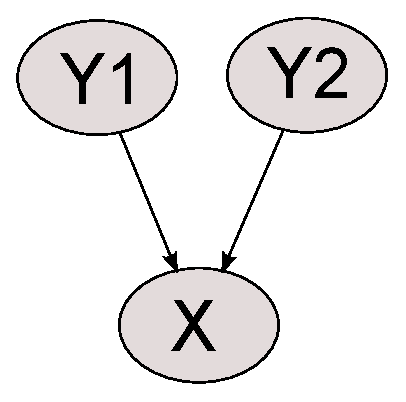
\includegraphics{img/bn1.eps}
\caption{Bayesian network with random variables $Y_1$, $Y_2$ and $X$. $Y_1$ and $Y_2$ are independent, while $X$ depends on $Y_1$ and $Y_2$.}
\label{bn1}
\end{figure}



\subsection{Conditional Probability Distribution}
Conditional Probability Distribution, or CPD, are modelling a conditional probability $p$, of a random variable $X$ given the parents $Y$ as following: $p(X|Y)$. $Y$ can represent several random variables. Each CPD has a scope composed of the variables it contains (i.e., $(X,Y)$). Inference and learning algorithms for bayesian network will require the CPD to implement some basic operations such as:
\begin{compactitem}
\item marginalization: given $p(X,Y)$, compute $p(X)$,
\item conditioning: given $p(X,Y)$ and evidence $Y=y$, compute $p(X,Y=y)$,
\item normalization: given $p(X)$, update the CPD so that it represents a probability distribution,
\item multiplication: given $p(X)$ and $p(Y)$ combine the CPDs into a joint distribution $p(X,Y)$
\end{compactitem}

To simplify the implementation, the scope will be identified by an integer with the following properties:
\begin{compactitem}
\item the parents' identifier will be higher than the children's identifier,
\item the scope of the CPD will always be sorted according to the identifier in increasing order. Consequently Scope[0] will always be the children variables.
\end{compactitem}

\subsubsection{Table Factor \nllref{PotentialTable}}
A table CPD is encoding probabilities for random discrete variables in a dense way. Given a random variable $X$ with $N$ Parents $Par_i(X)$, the table will have a size of $Size=\counta{X}\prod_{n=1}^{N} \counta{Par_n(X)}$. The table will consider the scope as a new basis so that $index(X_1=e_1, ..., X_n=e_n)=\sum_{j=1}^N e_j \prod_{i=1}^{j-1}\counta{X_i} $. For example, see the table CPD of Figure \ref{tablecpd1}.

\begin{table}[h]
\label{tablecpd1}
\centering
\begin{tabular}{| l | l |}
\hline
$p(X_2, X_1)$ & index\\
\hline\hline
(0, 0) & 0\\
\hline
(0, 1) & 1\\
\hline
(1, 0) & 2\\
\hline
(1, 1) & 3\\
\hline
(2, 0) & 4\\
\hline
(2, 1) & 5\\
\hline
\end{tabular}
\caption{Table CPD encoding the conditional distribution $p(X_1|X_2)$ or joint distribution $p(X_1,X_2)$ of two discrete random variables $X_1$ and $X_2$ of cardinality 2 and 3 respectively.}
\end{table}


\begin{compactitem}
\item marginalization: given $p(X,Y)$ compute $p(X) = \sum_{y_i \in Y}p(X)p(X|Y=y_i)$,
\item conditioning: $p(X,Y=y)$ simply eliminates the rows that do not agree with $y$ and drop $Y$ from the scope,
\item normalization: normalize the table so that $\sum_ip(X=i)=1$,
\item scope extension: given $p(X)$, extend the CPD's scope to $(X, Y)$ such that $p(X=i|Y_j) = p(X=i), \forall j$
\item multiplication: given $p(X)$ and $p(Y)$ merge the CPD into a single CPD $p(X,Y)$. First extend $p(X)$ scope to $Y$ (and similarly for $p(Y)$), then multiply the tables element by element.
\end{compactitem}

\subsubsection{Gaussian Moment Factor \nllref{PotentialGaussianMoment}}
\subsubsubsection{Parametrization}
Consider a Gaussian with mean $\mu$ and covariance matrix $\Sigma$ defined on some domain $x$ of size $n$.
\begin{align*}
\phi(x; \alpha, \mu, \Sigma) = \alpha  e^{-\frac{1}{2}(x-\mu)^T\Sigma^{-1}(x-\mu)}
\end{align*}
If $\alpha = (2\pi)^{-n0.5} \Sigma^{-0.5}$, the potential is exactly a gaussian PDF and will be called "normalized". Note that in most published papers, $\alpha$ will often be wrongly computed and this is why the computations are extensively detailed.

\subsubsubsection{Block diagonalization}
Consider a general partitioned matrix $M= \left[ \begin{array}{cc} E & F \\ G & H \end{array} \right]$ To zero out the upper right and lower left part of the matrix, we can do the following:

%% see http://people.csail.mit.edu/yks/documents/classes/mlbook/pdf/chapter12.pdf
%% and http://vis.uky.edu/~cheung/courses/ee595/MultivariateGaussian.ppt
$$
\left[ \begin{array}{cc} I & -FH^{-1} \\ 0 & I \end{array} \right]
\left[ \begin{array}{cc} E & F \\ G & H \end{array} \right]
\left[ \begin{array}{cc} I & 0 \\ -H^{-1}G & I \end{array} \right]
=
\left[ \begin{array}{cc} E-FH^{-1}G & 0 \\ 0 & H \end{array} \right]
$$

We define the Schur complement of matrix M with respect to H, $M/H = E-FH^{-1}G$. Since $(XYZ)^{-1}=Z^{-1}Y^{-1}Z^{-1}=W^{-1}$ and so $Y^{-1}=ZW^{-1}X$. Consequently we have:
\begin{align}
\left[ \begin{array}{cc} E & F \\ G & H \end{array} \right]^{-1}
&=
\left[ \begin{array}{cc} I & 0 \\ -H^{-1}G & I \end{array} \right]
\left[ \begin{array}{cc} (M/H)^{-1} & 0 \\ 0 & H^{-1} \end{array} \right]
\left[ \begin{array}{cc} I & -FH^{-1} \\ 0 & I \end{array} \right] \nonumber\\
&=
\left[ \begin{array}{cc} (M/H)^{-1} & -(M/H)^{-1}FH^{-1} \\
-H^{-1}G(M/H)^{-1} & H^{-1}+H^{-1}G(M/H)^{-1}FH^{-1} \end{array} \right] \label{blockinv}
\end{align}
Note that we can also decompose the matrix as followed:
$$
\left[ \begin{array}{cc} I & 0 \\ -GE^{-1} & I \end{array} \right]
\left[ \begin{array}{cc} E & F \\ G & H \end{array} \right]
\left[ \begin{array}{cc} I & -E^{-1}F \\ 0 & I \end{array} \right]
=
\left[ \begin{array}{cc} E & 0 \\ 0 & -GE^{-1}F - H \end{array} \right]
$$
Which similarly to (\ref{blockinv}) lead to the following:
\begin{align}
\left[ \begin{array}{cc} E & F \\ G & H \end{array} \right]^{-1}
&=
\left[ \begin{array}{cc} E^{-1} + E^{-1}F(M/E)^{-1}GE^{-1} & -E^{-1}F(M/E)^{-1} \\ -(M/E)^{-1}GE^{-1} & (M/E)^{-1} \end{array} \right] \label{blockinv2}
\end{align}
We can note that $|M|=|M/H||H|$.

~\\ \subsubsubsection{Marginalization}
%Consider a Gaussian on some domain $(x_1, x_2)$ of size $(p,q)$ with mean $\mu = \left[ \begin{array}{c} \mu_1 \\ \mu_2 \end{array} \right]$ and covariance $\Sigma = \left[ \begin{array}{cc}
Consider a Gaussian on some domain $(x_1, x_2)$ of size $(p,q)$ with mean $\mu = \left[ \mu_1~\mu_2 \right]^T$ and covariance $\Sigma = \left[ \begin{array}{cc} \Sigma_{11} & \Sigma_{12} \\ \Sigma_{21} & \Sigma_{22} \end{array} \right]$. We have:
\begin{align*}
&p(x_1,x_2)=
\underbrace{
\frac{1}{(2\pi)^{1/2*(p+q)}|\Sigma|^{1/2k}}
}_A
\exp
\underbrace{
\left\{
  -\frac{1}{2}
  \left( \begin{array}{c} x_1 - \mu_1 \\ x_2 - \mu_2 \end{array} \right)^{T}
  \left[ \begin{array}{cc} \Sigma_{11} & \Sigma_{12} \\ \Sigma_{21} & \Sigma_{22} \end{array} \right]^{-1}
  \left( \begin{array}{c} x_1 - \mu_1 \\ x_2 - \mu_2 \end{array} \right)
\right\}
}_B \\
B &=
\left\{
  -\frac{1}{2}
  \left( \begin{array}{c} x_1 - \mu_1 \\ x_2 - \mu_2 \end{array} \right)^{T}
  \left[ \begin{array}{cc} I & 0 \\ -\Sigma_{22}^{-1}\Sigma_{21} & I\end{array} \right]
  \left[ \begin{array}{cc} (\Sigma/\Sigma_{22})^{-1} & 0 \\ 0 & \Sigma_{22}^{-1} \end{array} \right]
  \left[ \begin{array}{cc} I & -\Sigma_{12}\Sigma_{22}^{-1} \\ 0 & I\end{array} \right]
  \left( \begin{array}{c} x_1 - \mu_1 \\ x_2 - \mu_2 \end{array} \right)
\right\}\\
&= -\frac{1}{2} %\left\{
(x_1 - \mu_1-\Sigma_{12}\Sigma_{22}^{-1}(x_2-\mu_2))^T(\Sigma/\Sigma_{22})^{-1}(x_1 - \mu_1-\Sigma_{12}\Sigma_{22}^{-1}(x_2-\mu_2))\\
&~~~-\frac{1}{2} (x_2-\mu_2)^T\Sigma_{22}^{-1}(x_2-\mu_2)\\
A &= \frac{1}{(2\pi)^{0.5(p+q)}(|\Sigma/\Sigma_{22}||\Sigma_{22}|)^{0.5}}\\
&= \left(
     \frac{1}{(2\pi)^{0.5p}|\Sigma/\Sigma_{22}|^{0.5}}
   \right)
   \left(
     \frac{1}{(2\pi)^{0.5q}|\Sigma_{22}|^{0.5}}
   \right)
%\right\}
\end{align*}


From the relation $p(x_1,x_2) = p(x_1|x_2)p(x_2)$ and the previous equations, we find that:
\begin{align*}
p(x_2) &= \frac{1}{(2\pi)^{0.5q}|\Sigma_{22}|^{0.5}} \exp \left( -\frac{1}{2} (x_2 - \mu_2)^T \Sigma_{22}^{-1} (x_2 - \mu_2)\right)\\
p(x_1|x_2) &= \frac{1}{(2\pi)^{0.5p}|\Sigma/\Sigma_{22}|^{0.5}}* \\ ~~~~& \exp \left(
                                                                     -\frac{1}{2}
(x_1 - \mu_1-\Sigma_{12}\Sigma_{22}^{-1}(x_2-\mu_2))^T(\Sigma/\Sigma_{22})^{-1}(x_1 - \mu_1-\Sigma_{12}\Sigma_{22}^{-1}(x_2-\mu_2))
                                                                     \right)
\end{align*}

Note that we extend the previous results for non-normalized gaussian distribution which gives us the following results:
\begin{align*}
\phi(x_2) &= \int \phi(x_1,x_2)dx_1\\
&= \phi(x_2; \alpha, \mu_2, \Sigma_2)\int p(x_1|x_2)dx_1\\
&= \phi(x_2; \frac{\alpha}{\alpha_{1|2}}, \mu_2, \Sigma_2) \text{~where~} \alpha_{1|2} = \frac{1}{(2\pi)^{0.5p}|\Sigma/\Sigma_{22}|^{0.5}}
\end{align*}

~\\ \subsubsubsection{Conditioning}
Suppose we are observing $x_2$ with value $\hat{x}_2$, then we have:
\begin{align*}
\phi(x_1, x_2=\hat{x}_2)&=\alpha \exp \left( B \right)\\
&= \phi( x_1; \alpha\alpha_2, \mu_1 + \Sigma_{12}\Sigma_{22}^{-1}(\hat{x}_2 - \mu_2), \Sigma_{11} + \Sigma_{12}\Sigma_{22}^{-1}\Sigma_{21} )
\end{align*}
Where $\alpha_2=\exp \left( - \frac{1}{2}\hat{x}_2^T\Sigma_{22}^{-1}\hat{x}_2 \right)$

\subsubsection{Gaussian Canonical Factor}
\subsubsubsection{Parametrization}
Unfortunately multiplication operations are difficult to realize in the moment form as it involves the inversion of the two potentials' covariance matrices which may not exist. To help with this, the computation will be done on another form, namely the canonical representation.
$$
\phi(x; K, h, g) = \exp(g+h^Tx - \frac{1}{2}x^TKx)
$$

\subsubsubsection{Moment to Canonical representation}
\begin{align*}
\phi(x; \alpha, \mu, \Sigma) &= \alpha \exp ( -\frac{1}{2} (x-\mu)^T\Sigma^{-1}(x-\mu)) \\
&= \exp ( \log (\alpha) - \frac{1}{2}(x^T\Sigma^{-1}x
                                     -x^T\Sigma^{-1}\mu
                                     -\mu^T\Sigma^{-1}x
                                     +\mu^T\Sigma^{-1}\mu
                                      ))\\
&= \exp ( \{\log (\alpha) - \frac{1}{2}\mu^T\Sigma^{-1}\mu\} + \{(\Sigma^{-1}\mu)^T x\} + \{x^T\Sigma^{-1}x\} )
\end{align*}

We conclude that:
\begin{align}
K &= \Sigma^{-1}\\
h &=\Sigma^{-1}\mu\\
g &= \log (\alpha) - \frac{1}{2}\mu^T\Sigma^{-1}\mu
\end{align}

\subsubsubsection{Canonical to Moment representation}
\begin{align}
\Sigma &= K^{-1}\\
\mu &=K^{-1}h \label{meanhCanonical}
\end{align}
Additionally we have:
\begin{align}
g&= \log (\alpha) - \frac{1}{2}(K^{-1}h)^TK^{-1}h \nonumber\\
&= \log (\alpha) - \frac{1}{2}h^TK^{-1}h \nonumber\\
\log (\alpha) &= g + \frac{1}{2}h^TK^{-1}h \nonumber\\
\alpha &= \exp(g + \frac{1}{2}h^TK^{-1}h )
\end{align}

\subsubsubsection{Multiplication/Division}
When multiplied, potentials are first extended to the other's domain by adding zeros. Multiplying/Dividing potentials in exponential forms is straightforward:
\begin{align}
\phi(K_a, h_a, g_a)*\phi(K_b, h_b, g_b) = \phi(K_a + K_b, h_a + h_b, g_a + g_b)\\
\phi(K_a, h_a, g_a)/\phi(K_b, h_b, g_b) = \phi(K_a - K_b, h_a - h_b, g_a - g_b)
\end{align}

\subsubsubsection{Marginalization}
Consider the potential:
$$
\phi(x_1, x_2) = \left[ \left( \begin{array}{c} h_1 \\ h_2 \end{array} \right), \left[ \begin{array}{cc} K_{11} & K_{12} \\ K_{21} & K_{22} \end{array} \right], g \right]
$$
We want to find:
\begin{align*}
\phi(x_1; h', K', g') &= \int \phi(x_1, x_2)dx_2\\
&= \int \phi(x_1; h', K', g)p(x_2|x_1)dx_1\\
&= \phi(x_1; h', K', g)\int p(x_2|x_1)dx_1
\end{align*}

By definition, we have:
$$
\left[ \begin{array}{cc} K_{11} & K_{12} \\ K_{21} & K_{22} \end{array} \right]^{-1} = \left[ \begin{array}{cc} \Sigma_{11} & \Sigma_{12} \\ \Sigma_{21} & \Sigma_{22} \end{array} \right]
$$
Using (\ref{blockinv}) we find that 
$$\bm{K'=K_{11}=(\Sigma/\Sigma_{22})^{-1} = K_{11}-K_{12}K_{22}^{-1}K_{21}}$$
Using (\ref{blockinv2}) we have:
\begin{align}
K_{22} &= (\Sigma/\Sigma_{11})^{-1}\nonumber\\
K_{12} &= - \Sigma_{11}^{-1}\Sigma_{12}(\Sigma/\Sigma_{11})^{-1}\nonumber\\
&= - \Sigma_{11}^{-1}\Sigma_{12}K_{22}\nonumber\\
\text{meaning~that~} \Sigma_{12} &= -\Sigma_{11}K_{12}K_{22}^{-1}\label{marg1}
\end{align}

Using (\ref{meanhCanonical}) we have:
\begin{align*}
\left( \begin{array}{c} \mu_1 \\ \mu_2 \end{array} \right) &=
\left[ \begin{array}{cc} \Sigma_{11} & \Sigma_{12} \\ \Sigma_{21} & \Sigma_{22} \end{array} \right] \left( \begin{array}{c} h_1 \\ h_2 \end{array} \right) \\
\mu_1 &= \Sigma_{11}h_1 +  \Sigma_{12}h_2\\
\text{By definition~}h'&= \Sigma_{11}^{-1}\mu_1 \\
\text{Injecting~}\mu_1~h' &=\Sigma_{11}^{-1}(\Sigma_{11}h_1 +  \Sigma_{12}h_2)\\
\text{Using (\ref{marg1}) we find that~}\bm{h'} &= \bm{h_1 -K_{12}K_{22}^{-1}h_2}
\end{align*}

Finally, we compute the constant in the same way as we did for the moment case. We use $\alpha_2$ as the normalization constant for $p(x_2)$:
\begin{align*}
\phi(x_1) &= \int \phi(x_1,x_2)dx_2\\
&= \int \phi(x_1; h', K', g)p(x_2|x_1)dx_1\\
&= \phi(x_1; h', K', g)\int p(x_2|x_1)dx_1\\
&= \bm{\phi(x_1; h', K', g-(\log(\alpha_2)-\frac{1}{2}\mu_2^T \Sigma_{22}^{-1}\mu_2)}\\
~\text{With~}&\alpha_2=\frac{1}{(2\pi)^{0.5q}|\Sigma_{22}|^{0.5}}
\end{align*}

\subsubsubsection{Conditioning}
Suppose we are observing $x_2$ with value $\hat{x}_2$, then we have:
\begin{align*}
\phi(x_1, x_2=\hat{x}_2) &= \exp\left( g + \left( \begin{array}{c} h_1 \\ h_2 \end{array}\right)^T
                                           \left( \begin{array}{c} x_1 \\ \hat{x}_2 \end{array}\right)
- \frac{1}{2} \left( \begin{array}{c} x_1 \\ \hat{x}_2 \end{array}\right)^T
              \left[ \begin{array}{cc} K_{11} & K_{12} \\ K_{21} & K_{22} \end{array} \right]
              \left( \begin{array}{c} x_1 \\ \hat{x}_2 \end{array}\right)
                                        \right)\\
&= \exp \left(
              \left\{ g + h_2^T\hat{x}_2 - \frac{1}{2}\hat{x}_2^T K_{22} \hat{x}_2 \right\} +
              \left\{ x_1^T(h_1-K_{12}\hat{x}_2) \right\} +    
              \left\{ -\frac{1}{2}x_1^T K_{11}x_1 \right\}
        \right)
\end{align*}

\subsubsection{Linear Gaussian Factor}
\lglossary{LG}{Linear Gaussian}
Let $y$ be a continuous node with continuous parents $x_1...x_k$. We says that $y$ has a linear Gaussian model if it can be described using parameters $\beta_0...\beta_k$ and $\sigma$ such that:
$$
P(y|x_1, ..., x_k)=N(\mu_u + \beta_1x_1 + ... + \beta_kx_k; \sigma^2)
$$


\subsubsection{Conditional Linear Gaussian Factor}
\lglossary{CLG}{Conditional Linear Gaussian}

We are building on top of the Linear Gaussian CPD (LG), where discrete parents of continuous variables are allowed in the model. We are facing two problems:
\begin{compactitem}
\item if we marginalize a discrete variable of a CLG, the resulting PDF will be a mixture of gaussians of higher dimension than each of the LG it is composed of,
\item we cannot represent CLG with a discrete variable having a gaussian parent
\end{compactitem}

\subsubsection{Mixture of truncated exponentials}
\lglossary{MTE}{Mixture of truncated exponentials}

\subsubsection{Always Observed Nodes}
If we can guaranty that some variables are always observed then we can easily combine any model in the bayesian network (neural nets, trees...) as we do not need to manipulate its PDF.

\subsection{Inference}
\subsubsection{Naive algorithm}
The naive algorithm is an exact inference algorithm. It simply constructs the full joint probability after incorporating the evidence to form the result of the inference query. Since it is extremely simple but generally inefficient (except for the Gaussian or Linear Gaussian CPD) it is only used for debugging purposes.

\subsubsection{Variable elimination}
\subsection{Learning}
\subsubsection{Fully observed case}

\section{Other Algorithms}
\subsection{k-means clustering \nllref{KMeans}}
k-means clustering is a method of cluster analysis which aims to partition $N$ observations into $K$ clusters $c_k$ in which each observation belongs to the cluster with the nearest mean.

We want to determine:
\begin{align}
\min_{c_k,r_{ik}} D &= \sum_{i=1}^N\sum_{k=1}^K r_{ik} \norm{x_i-c_k}^2\nonumber\\
\frac{\partial}{\partial c_k}D &= 2 \sum_{i=1}^Nr_{ik}(x_i-c_k) \nonumber\\
c_k &= \frac{\sum_{i=1}^N r_{ik}x_i}{\sum_{i=1}^N r_{ik}} \label{kmeansUpdate}
\end{align}

With $r_{ik}=1$ if the point $i$ belongs to cluster $k$, 0 otherwise. The algorithm repeats these two steps until convergence:
\begin{compactitem}
\item assign $r_{ik}$ so that each point belongs to the closest cluster
\item update the cluster position using \ref{kmeansUpdate}
\end{compactitem}
It must be noted that the algorithm is very sensitive to the initial cluster position.
\subsection{Hessian approximation FD \nllref{HessianCalculatorForwardFiniteDifference}}
Using finite differences, we have:
\begin{align}
\frac{\partial f(x)}{\partial x_i \partial x_j} &= \frac{\partial}{\partial x_j}( \frac{\partial f(x)}{x_i}) \nonumber\\
&= \frac{\partial}{\partial x_j}( \frac{f(x + he_i) - f(x)}{h} ) \nonumber\\
&= \frac{1}{h}( \frac{f(x + he_i + he_j) - f(x + he_i)}{h} - \frac{f(x + he_j) - f(x)}{h} ) \nonumber\\
&= \frac{f(x + he_i + he_j) - f(x + he_i)-f(x + he_j)+f(x)}{h^2}
\end{align}

with $h$ close to 0 and $e_k$ the basis vector for the parameter $k$. See~\cite{Scolnik01} for other implementations and drawbacks. Note that the step size $h$ must be sufficiently low for a good accuracy but it must be as well sufficiently high to avoid underflow problems; This is problem dependent.

\section{Optimization algorithms}
\subsection{Newton's method \nllref{OptimizerNewton}}
The Newton's method finds a \textbf{local extremum} (i.e., minimum or maximum) by constructing a sequence $x_n$ from an initial guess $x_0$ that converges towards $x_*$ such that the function $\nabla_f(x_n)=0$. Consequently finding a global extremum is not guaranteed. The closer the initial guess is from the global extremum, the more likely it is to find the global extremum.

It is assuming the function $f$ is twice differentiable and locally approximated well by a quadratic function. The function $f$ is locally approximated by a Taylor series of degree two:
\begin{align}
f(x_n + p)&= f(x_n) + p^T \nabla_f(x_n) + \frac{1}{2} p^T H_f(x_n) p + \bigO(p^3) \nonumber\\
\frac{d}{dp}f(x_n) &= 0 \nonumber\\
\frac{d}{dp}f(x_n) &=\nabla_f(x_n) + H_f(x_n) p \nonumber\\
p &= H_f^{-1}(x_n) \nabla{f}(x_n) \nonumber\\
\text{taking~} p = x_{n+1} - x_n \nonumber
&\text{~we obtain~} x_{n+1} = x_n - H_f^{-1}(x_n) \nabla{f}(x_n)
\end{align}

Additionally, the iteration step is scaled by $\gamma \in ]0..1]$ to help with the convergence, leading to the following update:
\begin{align}
x_{n+1} = x_n - \gamma H_f^{-1}(x_n) \nabla{f}(x_n) \label{newtonstep}
\end{align}

In the case $H_f$ is not invertible, the hessian matrix is reconditioned such that $H_f~=~H_f~+~\lambda I$, with $\lambda$ a small value. Note that since we are inverting the Hessian matrix as in (\ref{newtonstep}), this algorithm is not suitable for functions with a high number of variables.

\subsection{Gradient Descent \nllref{OptimizerGradientDescent}}
The Newton's method is attempting to construct a sequence $x_n$ from an initial guess $x_0$ that converges towards $x_*$ such that the function $\nabla_f(x_n)=0$. Consequently finding a global extremum is not guaranteed. The closer the initial guess is from the global minimum, the more likely it is to find the global minimum.

It is assuming the function $f$ is differentiable. The parameters must be properly scaled (i.e., all the parameters are comparable and none of them is dominating the others). The update is simply:
\begin{align}
x_{n+1} = x_n - \lambda \nabla{f}(x_n) \label{gradientstep}
\end{align}
$\lambda$ must be sufficiently small to avoid the bouncing effect and sufficiently by for fast convergence. $\lambda$ is a single value if the parameters are scaled or can be a vector so that each parameter is scaled independently. The gradient can be normalized to have more comparable $\lambda$ accross problems.

If the parameters are not properly scaled (e.g., narrow valley), convergence may be extremely slow. In this case a second order method is advised.

\subsection{Hybrid Gradient Descent \nllref{OptimizerGradientDescentLineSearch}}
One problem with the Gradient Descent is that the step size $\lambda$ is constant (it might be a good step at the beginning of the optimization, but not so afterward) and needs to be chosen by hand with all the problems that implies. An alternative is to have a variable step size and its value being computed by a line search. Note that this approach requires more function evaluations. This leads to the following parameter update:

\begin{align}
& d_n = \frac{\nabla{f}(x_n)}{\lVert \nabla{f}(x_n) \lVert} \nonumber\\
& \lambda_n = lineSearch(x_n, d_n) \nonumber\\
& x_{n+1} = x_n - \lambda _n d_n
\end{align}

If the parameters are not properly scaled (e.g., narrow valley), convergence may be extremely slow. In this case a second order method is advised.

Very similarly, other optimizers are combined with a line search such as
\nllref{OptimizerNewtonLineSearch}

\subsection{Grid Search \nllref{OptimizerGridSearch}}
Find the optimal parameters using an exhaustive search at discrete intervals. The search step for each parameter is defined
by \textbf{param.next(currentVal)}. Grid search could be extremely expensive in time, but it is guaranteed that it will find the minimum
value on this grid. If the evaluation function is quite fast, and the range search is small, this algorithm is suitable. It is often used for parameter selection for example for a classifier.

\subsection{Harmony Search \nllref{OptimizerHarmonySearch}}
Harmony search (HS) is a meta-heuristic optimization method imitating the music improvisation process where
musicians improvise their instruments' pitches searching for a perfect state of harmony. The following inputs are required:
\begin{compactitem}
\item hms: harmony memory rate. The memory size used to improvise new harmony from. Typical range is [10..100],
\item hmrc: harmony considering rate. Indicates the probability of generating a value from the memory. Typical range is [0.7..0.99],
\item par: pitch adjusting rate. Given a value generated from memory, this indicates the probability of modifying it. [0.1..0.4],
\item bw: bandwith. The update size,
\item f: the function to minimize.
\end{compactitem}

\begin{algorithm}
\caption{HarmonySearch(f, hms, hmrc, par, bw)}
\begin{algorithmic}
\STATE $memory \leftarrow InitializeRandomlyMemory(hms)$
\WHILE{$stoppingCriteria$}
\STATE // generate each value of vector from random,
\STATE // or taken from memory and slighly updated
\STATE $x \leftarrow empty$
\FOR{(i=0; n $<$ dim; ++n)}
\IF{$U(0,1)<hmrc$}
\STATE $x[i] \leftarrow memory[U(1..hms)][i]$
\IF{$U(0,1)<par$}
\STATE $x[i] \leftarrow x[i] \pm U(0..1) * bw$
\ENDIF
\ELSE
\STATE $x[i] \leftarrow random()$
\ENDIF
\ENDFOR
\STATE // finally evaluate the solution and remove
\STATE // from memory the worst one
\IF{$f(x) < memory.worst$()}
\STATE $memory.removeWorstAndAdd(x)$
\ENDIF
\ENDWHILE
\RETURN $memory.best()$

\end{algorithmic}
\end{algorithm}

\FloatBarrier

\subsection{Genetic Algorithm \nllref{OptimizerGeneticAlgorithm}}
The genetic algorithm (GA) optimizer uses a GA to perform the minimization. It is configured as following:
\begin{compactitem}
\item mutation operator: the value is randomly updated within the range of the parameter,
\item selection operator: elitist. The best solution is always selected and never mutated,
\item crossover operator: vector 2-point split. Two Potential solutions are selected and split at two random positions. Some segments of the solutions are swaped,
\item termination: defined by the number of epochs.
\end{compactitem}

\subsection{Powell's conjugate direction method \nllref{powell}}
The method minimises the function by a bi-directional search along each search vector, in turn. The new position can then be expressed as a linear combination of the search vectors. The new displacement vector becomes a new search vector, and is added to the end of the search vector list. Meanwhile the search vector which contributed most to the new direction, i.e. the one which was most successful, is deleted from the search vector list. The algorithm iterates an arbitrary number of times until no significant improvement is made. The function needs not be differentiable. Implemented exactly as described in \cite{NumericalRecipes}.


\subsection{Bracketing \nllref{minimumBracketing}}
Given a function $f$ and two initial points $a$ and $b$, find a triplet $(a', b', c')$ such that $f(a')>f(b')$ and  $f(c')>f(b')$. This is often to make sure that a function has at least a minima in this interval, especially for a line search algorithm. Implemented exactly as described in \cite{NumericalRecipes} using a golden section search.

\subsection{Line Search \nllref{lineMinimization}}
The line search is using \nllref{minimumBracketing} for an initial bracketing of the minimum followed by a line minimization, using brent's method which is a root-finding algorithm combining the bisection method, the secant method and inverse quadratic interpolation. It has the reliability of bisection but it can be as quick as some of the less reliable methods. The idea is to use the secant method or inverse quadratic interpolation if possible, because they converge faster, but to fall back to the more robust bisection method if necessary. The function needs not be differentiable. Implemented exactly as described in \cite{NumericalRecipes}.

\section{Classifiers}
\subsection{Feed Forward Neural Networks}
\subsection{Radial Basis Function Neural networks}
\subsection{Gaussian Mixture Models \nllref{gmm}}
\lglossary{GMM}{Gaussian Mixture Model}

A gaussian mixture model ($gmm$) is a generative model modelling a distribution using a mixture of gaussian models. It is defined as following $p(x|\Theta)= \sum_{k=1}^K \lambda _k N(x|\mu _k, \Sigma _k)$ Where $(\mu _k, \Sigma _k)$ is the parametrization of a gaussian and $\lambda _k$ its weight within the mixture.

Assuming we have $N$ samples $X=\{x_1,...,x_n\}$ which are independent and identically distributed, we have the log-likelihood function defined as:
\begin{align*}
L(\Theta | X)&=\log \prod_{i=1}^N p(x_i|\Theta) \\
&=\sum_{i=1}^N \log p(x_i|\Theta) \\
&=\sum_{i=1}^N \sum_{k=1}^K \log \lambda _k N(x_i|\mu _k, \Sigma _k) \\
\end{align*}

The log-likelihood is used as this is generally more stable numerically as it will avoid the overflow problem. We found that the parameters updates are:
\begin{align*}
\mu _ k &= \frac{1}{N_k} \sum_{i=1}^N \gamma _{ik} x_i \text{~with~} \\
\Sigma _k &= \frac{1}{N_k} \sum _{i=1}^N \gamma _{ik}(x_i-\mu _k)(x_i-\mu _k)^T \\
\lambda _k &= \frac{N_k}{N} \\
\end{align*}
With $N_k = \sum _{i=1}^N \gamma _{ik}$ and $\gamma _{ik} = \frac{\lambda_k N(x_i| \mu _k, \theta _k)}{\sum _{j=1}^K \lambda _j N(x_i| \mu _j, \theta _j)}$

~\\~
Initial values for $\lambda_k, \mu_k, \Sigma_k$ are found using K-means algorithm. For improved stability of the algorithm, $\Sigma_k$ is approximated by its diagonal (i.e., often if the number of mixture is too high, the matrix $\Sigma$ may not be invertible).

~\\~
In the classification context:
\begin{compactitem}
\item learning: for each class $k$, fit a $gmm_k$ with all the samples belonging to the class $k$.
\item classify: $class=\argmax_k L(x,\Theta_k)$
\end{compactitem}

\subsubsection{Derivation of the algorithm}
Recall that $\frac{d}{dx} \log f(x) = \frac{f'(x)}{f(x)}$ and $\frac{d}{dx} e ^x=x' e^x$, lets compute $\mu _k$:
\begin{align}
\frac{\partial L(\Theta | X)}{\partial\mu _k} &=  \sum_{i=1}^N \frac{\lambda_k N(x_i| \mu _k, \theta _k)}{\sum _{j=1}^K \lambda _j N(x_i| \mu _j, \theta _j)} \Sigma _k^{-1} (x_i-\mu _k) \nonumber\\
&=  \sum_{i=1}^N \gamma _{ik} \Sigma _k^{-1} (x_i-\mu _k) \text{~with ~} \nonumber\\
\text{rearranging~} \sum_{i=1}^N \gamma _{ik} \mu _ k &= \sum_{i=1}^N \gamma _{ik} x_i \nonumber\\
\bm{\mu _ k} &= \bm{\frac{1}{N_k} \sum_{i=1}^N \gamma _{ik} x_i} \text{~with~} N_k = \sum _{i=1}^N \gamma _{ik}
\end{align}

Recall that:
\begin{align*}
& \frac{d|M|}{dM} = |M|(M^{-1})^T \\
& \frac{d(a^TMb)}{dM} = ab^T
\end{align*}

Lets name $c=e^{-\frac{1}{2}(x_n-\mu_k)\Sigma_k(x_n-\mu_k)}$. We have:
\begin{align*}
\frac{\partial c}{\partial \Sigma^{-1}_k} &= c(-\frac{1}{2})(x_n - \mu_k)(x_n - \mu_k)^T \\
\frac{\partial \lambda_k N(x_n|\mu_k,\Sigma_k)}{\partial\Sigma_k^{-1}} &= \frac{\partial(\frac{\lambda_k|\Sigma_k^{-1}|^{0.5}}{(2 \pi)^{D/2}}c)}{\partial \Sigma^{-1}_k} \\
&= \frac{\lambda_k c}{(2 \pi)^{D/2}}\frac{\partial(|\Sigma_k^{-1}|^{0.5})}{\Sigma_k^{-1}}
+ \frac{\lambda_k |\Sigma_k^{-1}|^{0.5}}{(2 \pi)^{D/2}} \frac{\partial c}{\partial \Sigma_k^{-1}} \\
&=\frac{\lambda_k c}{(2 \pi)^{D/2}}\frac{1}{2}|\Sigma_k^{-1}|^{-1/2} |\Sigma_k^{-1}| \Sigma_k
+ \frac{\lambda_k |\Sigma_k^{-1}|^{0.5}}{(2 \pi)^{D/2}}c{(-0.5(x_n-\mu_k)(x_n-\mu_k)^T)}\\
&= \frac{1}{2} \frac{\lambda_k |\Sigma_k^{-1}|^{0.5}c}{(2 \pi)^{D/2}}(\Sigma_k - (x_n-\mu_k)(x_n-\mu_k)^T)\\
&= \frac{1}{2} N(x_n|\mu_k, \Sigma_k)(\Sigma_k - (x_n-\mu_k)(x_n-\mu_k)^T) \\
\frac{\partial ln p(X|\Theta)}{\partial \Sigma_k^{-1}} &= \sum_{n=1}^N
\frac{1}{\sum_{j=1}^K \lambda_k N(x_n|\mu_j,\Sigma_j)}
\frac{\partial \lambda_k N(x_n|\mu_k,\Sigma_k)}{\partial\Sigma_k^{-1}} \\
&= \frac{1}{2} \sum_{n=1}^N \frac{\lambda_k N(x_n|\mu_k,\Sigma_k)(\Sigma_k-(x_n-\lambda_k)(x_n-\lambda_k)^T))}{\sum_{j=1}^K \lambda_j N(x_n|\mu_j,\Sigma_j)}\\
&=\frac{1}{2}\sum_{n=1}^N\gamma_{nk}(\Sigma_k-(x_n-\lambda_k)(x_n-\lambda_k)^T))
\end{align*}
Setting $\frac{\partial ln p(X|\Theta)}{\partial \Sigma_k^{-1}}$ to 0, we get:
\begin{align*}
\bm{\Sigma _k} &= \bm{\frac{1}{N_k} \sum _{n=1}^N \gamma _{nk}(x_n-\mu _k)(x_n-\mu _k)^T}
\end{align*}

Finally, compute $\lambda_k$
\begin{align*}
\frac{\partial ln p(X|\Theta)}{\partial \mu_k^{-1}} &= \sum_{n=1}^K \frac{N(x_n|\mu_k,\Sigma_k)}{\sum_{j=1}^K N(x_j|\mu_j,\Sigma_j)} \\
&= \sum_{n=1}^K \frac{\gamma_{nk}}{\lambda_k} \text{~(i.e., we just add the missing term from~} \gamma_{nk})
\end{align*}
We need to consider the constraint $\sum_{k=1}^K \lambda_k=1$ and form the Lagrangian

\begin{align*}
L &=\ln p(X|\Theta) + \lambda((\sum_{k=1}^K \lambda_k-1)) \\
\frac{\partial L}{\partial \lambda_k} &= 0 \\
0 &= \sum_{n=1}^K \frac{\gamma_{nk}}{\lambda_k} - \lambda \\
\sum_{k=1}^K \sum_{n=1}^N \gamma_{nk} &= \lambda \sum_{n=1}^K( \lambda_K) \\
\sum_{n=1}^N 1 &= \lambda \\
\lambda &= N\\
\text{Substituting we have:~} \bm{\lambda_k} &= \bm{\frac{N_k}{N}}
\end{align*}
\subsection{Boosting}
\subsection{Decision Tree}
\subsection{Stump}
\subsection{Perceptron}

\section{Data Preprocessing}
\subsection{Feature Selection}
blabla
\subsubsection{Locally Linear Embedding}
\subsubsection{Pearson Correlation Ratio}
\subsubsection{Relief-f}
\subsubsection{Wrapper Methods}

\subsection{Feature Reduction}
\subsubsection{Principal Component Analysis}
\subsubsection{Kernel Principal Component Analysis}
\subsubsection{Independent Component Analysis}
\subsubsection{Principal Component Analysis}
\subsection{Normalization}


\section{3D Visualization Algorithms}
\subsection{Interpolators}
\subsubsection{Nearest Neighbour}
\subsubsection{Trilinear}
\subsection{Transformation Models}
\subsubsection{Affine}
\subsubsection{Radial Basis functions}
\subsubsection{Dense Deformable Field}
\subsection{Multi-Planar Reconstruction}
\subsection{Maximum Intensity Projection}

\section{Notations}
\begin{compactitem}
\item function~$f$ is defined throughout the document as $f \colon \textbf{R}^n \to \textbf{R}$
\item U(a..b) generate a random number uniformly in the range [a..b]
\item N(m, v) generate a random number following a gaussian distribution mean $m$ and standard deviation $v$
\item for a discrete random $X$, $\counta{X}$ will denote the number of states of $X$
\end{compactitem}

\printglossary

\bibliography{nll-algorithm-documentation}
\bibliographystyle{plain}

\end{document}
